\documentclass[aspectratio=169%可调屏宽比16:9(169),4:3(43)
,serif,mathserif]{beamer}
\mode<presentation>{
%\usetheme{default}
%\usetheme{AnnArbor}
%\usetheme{Antibes}
%\usetheme{Bergen}
%\usetheme{Berkeley}
%\usetheme{Berlin}
%\usetheme{Boadilla}
%\usetheme{CambridgeUS}
%\usetheme{Copenhagen}
%\usetheme{Darmstadt}
%\usetheme{Dresden}
%\usetheme{Frankfurt}
%\usetheme{Goettingen}
%\usetheme{Hannover}
%\usetheme{Ilmenau}
%\usetheme{JuanLesPins}
%\usetheme{Luebeck}
\usetheme{Madrid}
%\usetheme{Malmoe}
%\usetheme{Marburg}
%\usetheme{Montpellier}
%\usetheme{PaloAlto}
%\usetheme{Pittsburgh}
%\usetheme{Rochester}
%\usetheme{Singapore}
%\usetheme{Szeged}
%\usetheme{Warsaw}
% As well as themes, the Beamer class has a number of color themes
% for any slide theme. Uncomment each of these in turn to see how it
% changes the colors of your current slide theme.
%\usecolortheme{albatross}
%\usecolortheme{beaver}
%\usecolortheme{beetle}
%\usecolortheme{crane}
%\usecolortheme{dolphin}
%\usecolortheme{dove}
%\usecolortheme{fly}
%\usecolortheme{lily}
%\usecolortheme{orchid}
%\usecolortheme{rose}
%\usecolortheme{seagull}
%\usecolortheme{seahorse}
%\usecolortheme{whale}
%\usecolortheme{wolverine}
%\setbeamertemplate{footline} % To remove the footer line in all slides uncomment this line
%\setbeamertemplate{footline}[page number] % To replace the footer line in all slides with a simple slide count uncomment this line
%\setbeamertemplate{navigation symbols}{} % To remove the navigation symbols from the bottom of all slides uncomment this line
}
\usepackage{adjustbox}
\usepackage{indentfirst} 
\usepackage{amsmath, amsfonts, epsfig, xspace}
\usepackage{algorithm,algorithmic}
\usepackage{beamerthemesplit}
\usepackage{booktabs}
\usepackage{bm}
\usepackage{braket}
\usepackage{calligra}
\usepackage[T1]{fontenc}
\usepackage{fontspec}
\usepackage{ctex}
\usepackage{latexsym}
\usepackage{multicol}
\usepackage{multimedia}
\usepackage{calligra} \DeclareMathAlphabet{\mathcalligra}{T1}{calligra}{m}{n} \DeclareFontShape{T1}{calligra}{m}{n}{<->s*[2.2]callig15}{}
\usepackage{pstricks,pst-node}
\usepackage{ragged2e}
\usepackage{setspace}
\usepackage[normal,tight,center]{subfigure}
\setlength{\subfigcapskip}{-.5em}
\setlength{\parindent}{2em}
\begin{document}
\title{The Marabou Framework for Verification and Analysis of Deep Neural Networks} % The short title appears at the bottom of every slide, the full title is only on the title page
%\author[Chi~Zhiming]{迟智名} % Your name
\institute[ISCAS] % Your institution as it will appear on the bottom of every slide, may be shorthand to save space
{	
	%Lanzhou University \\ % Your institution for the title page
	%\medskip
	%\textit{chizhm16@lzu.edu.cn} % Your email address
}
	\CTEXoptions[today=old]
	\date{\today} % Date, can be changed to a custom date
\begin{frame}[plain]\vspace{1.5em}
\titlepage\vspace{-0.5cm}
%\centerline{\includegraphics[height=0.30\textheight]{logo.png}}
%\hfill 指导教师:xxx
\end{frame}
\begin{frame}{目录}
\tableofcontents
\end{frame}
\AtBeginSection[]
{
\begin{frame}{\tiny}
\frametitle{目录}
\tableofcontents[currentsection]
\end{frame}
}
%----------------------------------------------------------------------------------------
%	PRESENTATION SLIDES
%----------------------------------------------------------------------------------------

%------------------------------------------------
\section{Introduction} % Sections can be created in order to organize your presentation into discrete blocks, all sections and subsections are automatically printed in the table of contents as an overview of the talk
%------------------------------------------------
\begin{frame}
	\frametitle{Contribution}
	\begin{itemize}
		\item Marabou is an SMT-based tool that can answer queries about a network's properties by transforming these queries into constraint satisfaction problems.
		\item The Marabou framework is a significant improvement over its predecessor,
		Reluplex. Specifically, it includes the following enhancements and modifications: 
		\begin{itemize}
			\item support for CNN
			\item support for divide-and-conquer solving mode
			\item a simplex-based linear programming core that replaces the external solver (GLPK)
			\item Multiple interfaces for feeding queries into the solver
			\item Support for network-level reasoning and deduction.
		\end{itemize}
	\end{itemize}

\end{frame}

\section{Marabou}
\begin{frame}
	\frametitle{Design of Marabou}
	\begin{figure}[htbp]
		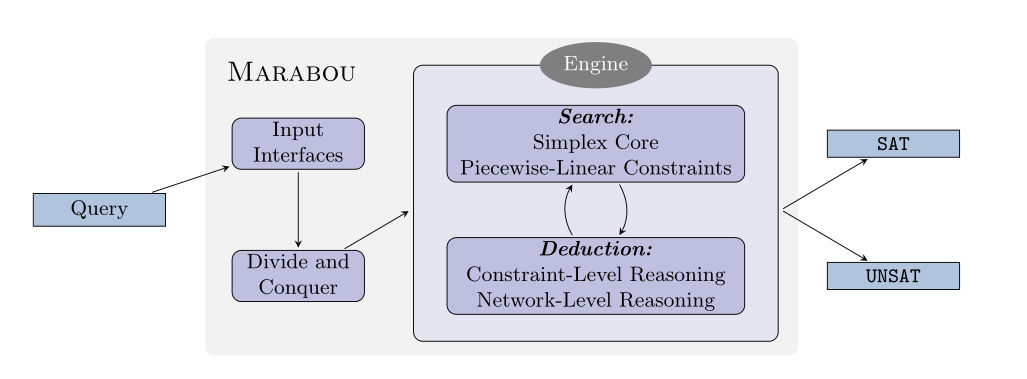
\includegraphics[width=1\linewidth]{1.png}
	\end{figure}
\end{frame}

\begin{frame}
	\frametitle{Simplex Core}
	\begin{itemize}
		\item Solve the linear constraints
		\item Reluplex: solve linear constraints by GLPK. $\to$ Marabou: implement a new custom solver 
			\begin{itemize}
				\item repeated translation of queries into GLPK and extraction of results from GLPK was a limiting factor on performance
				\item black box simplex solver did not afford the flexibility we needed in the context of DNN verification
			\end{itemize}		
	\end{itemize}	

\end{frame}

\begin{frame}
	\frametitle{Piecewise-Linear Constraints}
		
		\begin{itemize}
			\item configuration:
				\begin{itemize}
					\item abstract class: \textbf{PiecewiseLinearConstraint class}
					\item class: \textbf{Max} and \textbf{Relu}
					\item objects: constraints
				\end{itemize}
			\item methods of PiecewiseLinearConstraint class:
				\begin{itemize}
					\item \emph{satisfied()}
					\item \emph{getPossibleFixes()}
					\item \emph{getCaseSplits()}:piecewise-linear constraint $\varphi \to c_{1} \vee \ldots \vee c_{n}$
					\item \emph{getEntailedTightenings()}: query the constraint for tighter variable bounds
				\end{itemize}
		\end{itemize}
\end{frame}


\begin{frame}
	\frametitle{Constraint and Network-Level Reasoning}
	Constraint-level bound tightening: using \emph{getEntailedTightenings()}
	\begin{figure}[htbp]
		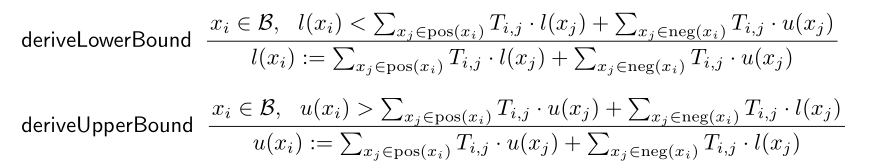
\includegraphics[width=1\linewidth]{3.png}
	\end{figure}
\end{frame}

\begin{frame}
	\frametitle{Constraint and Network-Level Reasoning}
	DNN-level reasoning: Symbolic interval propagation
	\begin{figure}[htbp]
		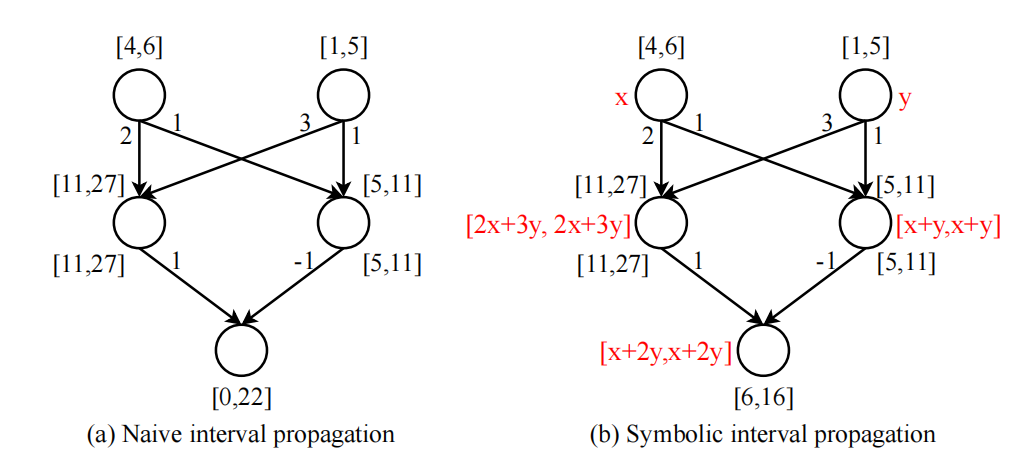
\includegraphics[width=0.9\linewidth]{2.png}
	\end{figure}
\end{frame}

\begin{frame}
	\frametitle{Constraint and Network-Level Reasoning}
	DNN-level reasoning:symbolic bound tightening procedure
	\begin{itemize}
		\item Initializing the DNN-level reasoners with the most up-to-date information discovered during the search, such as variable bounds and the state of piecewise-linear constraints
		\item Feeding any new information that is discovered back into the search procedure.
	\end{itemize}
\end{frame}

\begin{frame}
	\frametitle{Engine}
	\begin{columns}
		\begin{column}{.4\textwidth}
			\begin{figure}[htbp]
				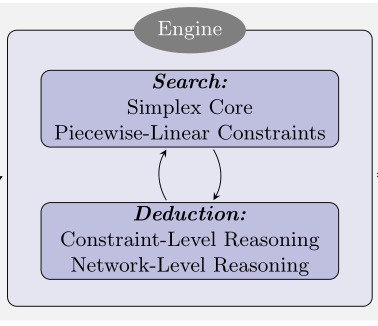
\includegraphics[width=1\linewidth]{4.png}
			\end{figure}
		\end{column}

		\begin{column}{.6\textwidth}
			\begin{itemize}
				\item If there is a violated linear constraint, perform a simplex step.
				\item If there is a violated piecewise-linear constraint, attempt to fix it.
				\item If a piecewise-linear constraint had to be fixed more than a certain number of times, perform a case split on that constraint.
				\item If the problem has become unsatisfiable, undo a previous case split (or return UNSAT if no such case split exists).

				\item  Return SAT (all constraints are satisfied).
				\item  Deduction: heuristics
			\end{itemize}
		\end{column}

	\end{columns}
\end{frame}



\begin{frame}
	\frametitle{The Divide-and-Conquer Mode and Concurrency}
	\begin{figure}[htbp]
		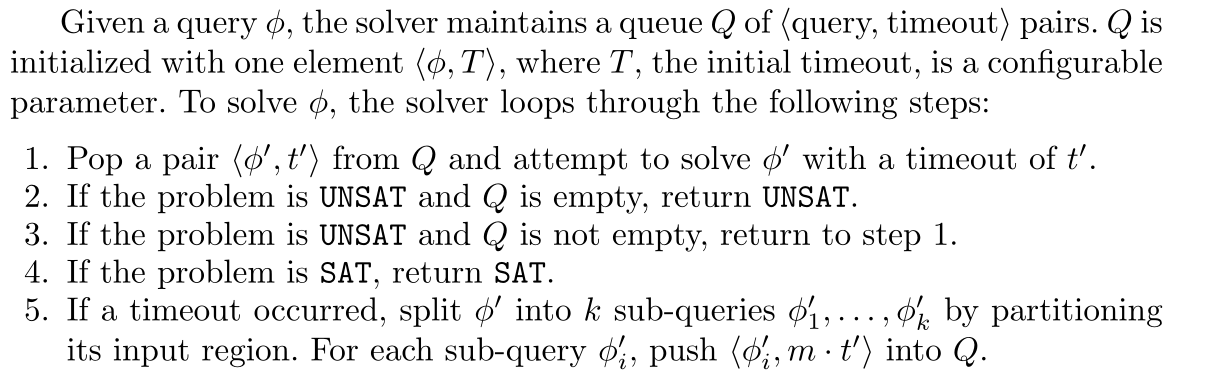
\includegraphics[width=1\linewidth]{6.png}
	\end{figure}
\end{frame}



%------------------------------------------------


%------------------------------------------------

%------------------------------------------------


%------------------------------------------------
\begin{frame}
\hfill
\center{\Huge{\calligra{\Huge{Thank you}}}}
\linespread{3}\selectfont
\end{frame}
%----------------------------------------------------------------------------------------
\end{document}